%! Author = charon
%! Date = 2/8/24

\subsection{Dokumentierte crashes, hangs und buggs}\label{subsec:dokumentierte-crashes-hangs-und-buggs}
Bevor auf die Crashes eingegangen wird, werden die im output Verzeichnis angelegten Daten und Verzeichnisse genauer erläutert.
\begin{figure}[h]
    \frame{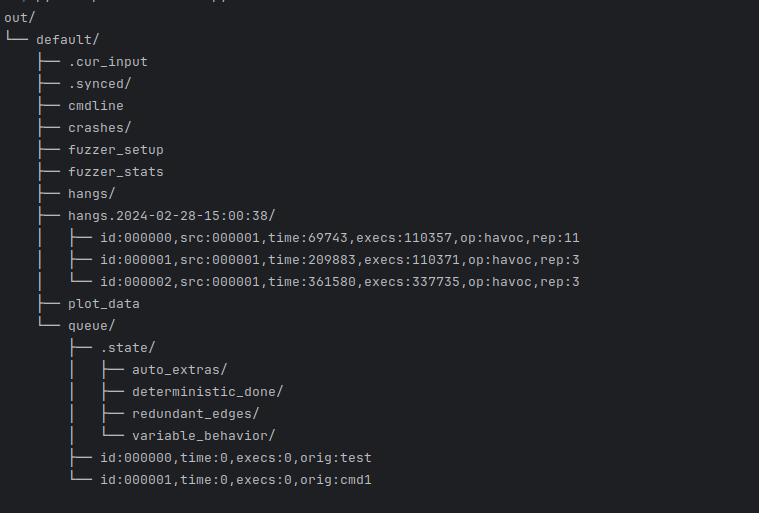
\includegraphics[width=\linewidth]{img/out-dir-structure}}
    \caption{Verzeichnisstruktur des output Verzeichnisses von AFL}\label{fig:out-dir-structure}
\end{figure}\\
Die drei Hauptverzeichnisse bestehen aus \textit{crashes/}, \textit{hangs/} und \textit{queue/}.
Bei dem Verzeichnis \textit{queue/} handelt es sich um den synthetischen Korpus.
Dieser wurde bei der Mutationsphase von~\gls{afl} mithilfe der bereitgestellten Testcases erstellt. \\
Die Verzeichnisse \textit{hangs/} und \textit{crashes/} existieren zur Dokumentation der durch Inputs verursachten Aufhängern
und Programmabstürzen.
Die jeweiligen Hangs und Crashes werden mit einer ~\gls{id} versehen, welche der numerisch sortierten chronologischen Reihenfolge
der Crashes entspricht.
Gefolgt werden sie von der Nummer des dafür verantwortlichen Inputs.
Der Inhalt der darin enthaltenen Daten entspricht dem Input, welcher das Programm zum Absturz oder Aufhängen gebracht hat.
Als Crash wird ein Fall bezeichnet, bei dem ein Input das Senden eines Signals wie \texttt{SIGSEGV} für \textit{segmentation fault}
und somit den Absturz des Programmes verursacht.
Hangs hingegen sind Fälle, welche das von ~\gls{afl} definierte Zeitlimit von einer Sekunde oder der selbst definierten
Zeitspanne -- mithilfe des \texttt{-t} Flags konfiguriert -- überschreiten.
Es wird zwischen einzigartigen und nicht einzigartigen Crashes und Hangs unterschieden.
Einzigartig sind diese nur, wenn der übermittelte Input einen zuvor unabgedeckten Codepfad überquert~\cite{inetpreting-output}. \\
Zur Zeit der Verfassung dieser Arbeit wurden in dem zu untersuchenden Binary \textit{mmapp} keine Crashes
mithilfe des~\gls{qemu} Modus gefunden. \\
\linebreak
Die Verifikation eines Crashes erfolgt durch das Ausführen des zu untersuchenden Programms mit dem Input, welcher
den Crash erzeugt hat.
Wenn der Crash mithilfe des Inputs reproduzierbar ist, so kann man sich den zugrundeliegenden \textit{code.dump} genauer
ansehen.
Im Fall eines segmentation faults liegt dann eine potenzielle Memory-Corruption-Schwachstelle vor.